Die Schwerpunkte $S_1$ und $S_2$ der beiden Rohre liegen in ihren Mitten. Die Massen der gleichartigen Rohre verhalten sich wie ihre Längen, $m_1 : m_2 = \lLaO : \lLbO = 2 : 3$. Der gemeinsame Schwerpunkt $S$ liegt auf der Verbindungsstrecke $S_1S_2$ und teilt sie umgekehrt im Verhältnis der Massen (Hebelgesetz):
\begin{align}
 m_1\cdot\overline{SS_1} &= m_2\cdot\overline{SS_2} \quad\Rightarrow\quad \overline{SS_2} : \overline{SS_1} = 2 : 3
\end{align}
Man teilt also die Strecke $S_1S_2$ in fünf gleiche Teile; $S$ liegt zwei Teile von $S_2$ und drei Teile von $S_1$ entfernt (Zeichnung im Massstab 1:5).

\begin{center}
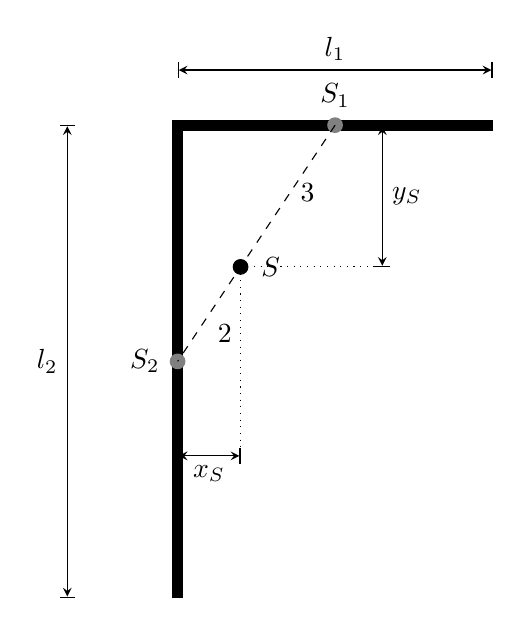
\begin{tikzpicture}[>=stealth]
 \draw[line width=4pt] (4,0) -- (0,0) -- (0,-6);
 \fill[gray] (2,0) circle (0.1) node[above=3pt, black] {$S_1$};
 \fill[gray] (0,-3) circle (0.1) node[left=3pt, black] {$S_2$};
 \draw[dashed] (2,0) -- (0,-3);
 \fill (0.8,-1.8) circle (0.1) node[right=4pt] {$S$};
 \node at (0.6,-2.65) {2};
 \node at (1.65,-0.85) {3};
 \draw[|<->|] (0,0.7) -- (4,0.7) node[midway, above] {$l_1$};
 \draw[|<->|] (-1.4,0) -- (-1.4,-6) node[midway, left] {$l_2$};
 \draw[dotted] (0.8,-1.8) -- (0.8,-4.2);
 \draw[|<->|] (0,-4.2) -- (0.8,-4.2) node[midway, below] {$x_S$};
 \draw[dotted] (0.8,-1.8) -- (2.6,-1.8);
 \draw[|<->|] (2.6,0) -- (2.6,-1.8) node[midway, right] {$y_S$};
\end{tikzpicture}
\end{center}

Rechnerisch (Ursprung in der Ecke, $x$ entlang des kurzen, $y$ entlang des langen Rohrs; Massen proportional zu den Längen):
\begin{align}
 x_S &= \frac{l_1\cdot\frac{l_1}{2} + l_2\cdot 0}{l_1+l_2} = \xLsF = \frac{\left(\lLa\right)^2}{2\cdot\left(\lLa+\lLb\right)} = \xLs \approx \result{\xLsP{-2}{2}} \\
 y_S &= \frac{l_1\cdot 0 + l_2\cdot\frac{l_2}{2}}{l_1+l_2} = \yLsF = \frac{\left(\lLb\right)^2}{2\cdot\left(\lLa+\lLb\right)} = \yLs \approx \result{\yLsP{-2}{2}}
\end{align}
Der Schwerpunkt liegt \xLsP{-2}{2} neben dem langen und \yLsP{-2}{2} neben dem kurzen Rohr, also ausserhalb des Materials im Winkel des L.
